\q{12}{Some More Regression}
\begin{enumerate}
    \vskip 0.2in
    \subq{3} The following depicts a scatter plot between two numerical variables (labeled \textit{x} and \textit{y}). A line (labeled "Line A") has been drawn through the scatter plot, but note that Line A is not the least squares regression line between x and y. \textbf{On the plot itself (do not make a separate plot), draw a line with a \textit{larger} root mean square error than the existing line.}
    \vskip 0.2in
    \begin{center}
        \solutionimage
        {
        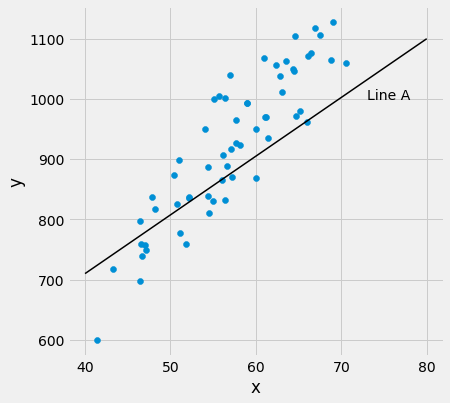
\includegraphics[scale=.45]{figures/labelledporpourri.png}
        }
        {
        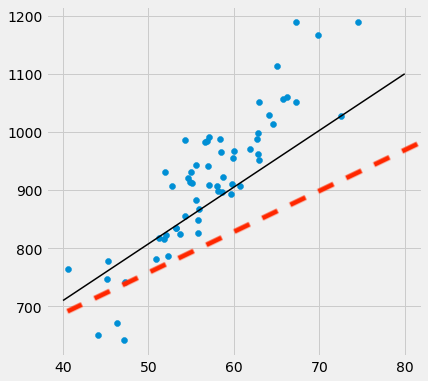
\includegraphics[scale=.45]{figures/potpourri_plot_sol.png}
        \solution{The line at left is one example of a valid answer.}
        }
    \end{center}
    
    
    

    \clearpage
    \subq{6} We have provided three empty plots, with axes in standard units. Draw a dataset of ten to twenty points with the specified value for \textit{r}. Make sure your points are clearly visible and large enough to see when scanned.\\[8pt]
    \textbf{Plot A:} Draw data points in a scatter plot such that the correlation of the points could be close to \textbf{0.}\\
    \textbf{Plot B:} Draw data points in a scatter plot such that the correlation of the points could be close to \textbf{0.99.}\\
    \textbf{Plot C:} Draw data points in a scatter plot such that the correlation of the points could be close to \textbf{-0.5.}\\
    \vskip 0.4in
    \solutionimage
    {
    \begin{tabular}{l@{\hskip 1in}l@{\hskip 0.1in}l@{\hskip 0.1in}l}
    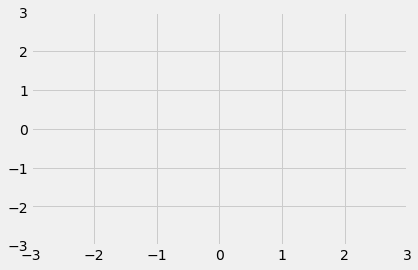
\includegraphics[scale=.45]{figures/blankaxes.png}
    &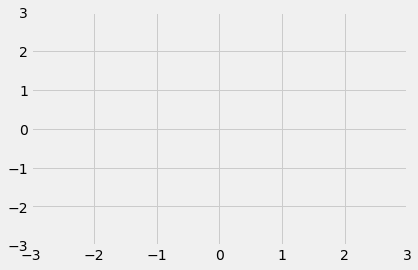
\includegraphics[scale=.45]{figures/blankaxes.png}\\
    {\hskip 1in}\textbf{Plot A}
    &{\hskip 1in}\textbf{Plot B}
    \end{tabular}
    \begin{center}
        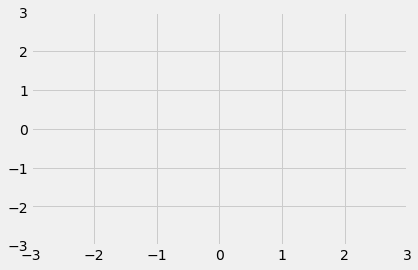
\includegraphics[scale=.45]{figures/blankaxes.png}\\
        \textbf{Plot C}
    \end{center}
    \solution{The points above are examples of valid solutions.}
    }
    {
    \begin{tabular}{l@{\hskip 1in}l@{\hskip 0.1in}l@{\hskip 0.1in}l}
    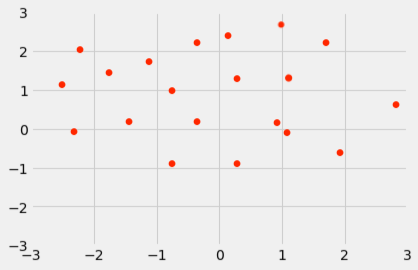
\includegraphics[scale=.45]{figures/corr0soln.png}
    &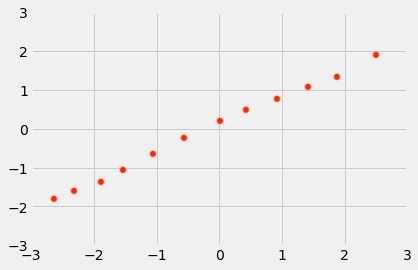
\includegraphics[scale=.45]{figures/corr099soln.png}\\
    {\hskip 1in}\textbf{Plot A}
    &{\hskip 1in}\textbf{Plot B}
    \end{tabular}
    \begin{center}
        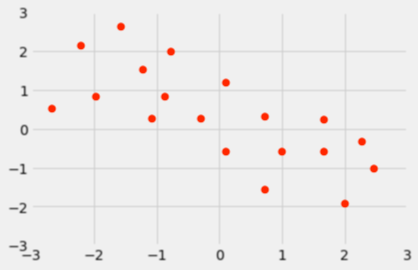
\includegraphics[scale=.45]{figures/corrneg05soln.png}\\
        \textbf{Plot C}
    \end{center}
    \solution{The points above are examples of valid solutions.}
    }
    \vskip 0.4in

    \subq{3} A researcher is interested in the relationship between the number of bumblebees and the number of ground squirrels observed in an alpine meadow over the course of one day. They calculate the regression line between the number of bees and the number of squirrels, and finds that the slope of the regression is 0.0314. Curious about the small value of the slope, the researcher wants to test the following hypotheses: 
    \begin{itemize}
        \item Null: The slope of the true line describing the relationship between number of bees and  number of squirrels in alpine meadows is zero. 
        \item Alternative: The slope of the true line describing the relationship between between number of bees and  number of squirrels in alpine meadows is not zero.
    \end{itemize}
The researcher finds that an  approximate 90\% confidence interval for the true slope is [0.013, 0.045]. Select \textbf{all} the p-value cutoffs for which the researcher will reject the null hypothesis:
\vskip 0.1in
\solutionbox 20\%\\
\solutionbox 10\%\\
\checkbox 5\%\\
\checkbox 1\%\\

\end{enumerate}